\chapter{Background}
\label{chap:Background}

\section{Messages}
\label{sec:messages}

In today's interconnected world, computer programs rarely exist in a vacuum.
Rather, they form one small part of a much larger \gls{soa} -
consisting of multiple services, jobs and scripts, all exchanging information in
the form of messages. These messages may adhere to a standard data-interchange
format (for example, \gls{json}). They may correspond to an agreed upon
specification (for example, \href{https://goo.gl/rjuP4C}{IEEE 1671-2010}).
Or they may simply be blobs of binary information transmitted over the network -
completely subject to the interpretation of the sender and received.
At a fundamental level, though, a message is simply a collection of bytes, to be
transmitted from point A, to point B.

\section{Message Brokers}
\label{sec:brokers}

\begin{figure}[ht]
  \centering
  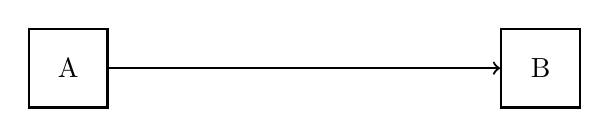
\begin{tikzpicture}[thick]
  \node(A) [draw,rectangle,minimum width=1cm,minimum height=1cm]{A};

  \begin{scope}[xshift=6cm]
    \node(B) [draw,rectangle,minimum width=1cm,minimum height=1cm]{B};
  \end{scope}

  \draw[->] (A) edge (B);
\end{tikzpicture}

  \caption{Two services, A and B, directly exchanging messages}
  \label{fig:tikz:directMessaging}
\end{figure}

To understand the role message brokers typically play in \glspl{soa}, we first
examine the simplest method of transmitting bytes between two applications -
directly transmitting messages between two applications (shown in
Figure~\ref{fig:tikz:directMessaging}).

In this example, the application 'A' wishes to transmit a simple message (a
sequence of bytes) to application 'B', and does so in the simplest method
possible. This could involve making an \gls{rpc}, opening a Unix/\gls{tcp}
socket, or making a HTTP web request - for the purposes of this illustration the
exact mechanism by which bytes are transferred is unimportant, the fact that the
transfer takes place \emph{directly} between the two parties is all that
matters.

\begin{figure}[ht]
  \centering
  \begin{tikzpicture}[thick]

  % Draw nodes
  \foreach \t [count=\a] in {A,B,C,D,E,F,G,H,I,J}{
    \draw (\a*360/10: 4cm) node(\t)[draw,rectangle,minimum width=1cm,minimum height=1cm]{\t};
    }

  % Draw connections
  \foreach \t [count=\a] in {A,B,C,D,E,F,G,H,I,J}{
    \foreach \u [count=\b] in {A,B,C,D,E,F,G,H,I,J}{
      \ifthenelse{\NOT \a=\b}{\draw[->] (\t) edge (\u)}{};
      }
    }

\end{tikzpicture}

  \caption{Ten services directly exchanging messages}
  \label{fig:tikz:complexDirectMessaging}
\end{figure}

This is a perfectly acceptable method of exchanging information between two
services at a small scale. However (and perhaps unfortunately), systems rarely
exist in pairs. One of the biggest issues with simple application-to-application
messaging is demonstrated in Figure~\ref{fig:tikz:complexDirectMessaging} - as
more nodes are added, the complexity of using direct connections increases
exponentially (requiring $n^2 - n$ connections, where $n$ is the number of
services)\footnote{Assuming each service needs to talk to all other services}.
Managing this complexity is difficult in a number of ways:

\begin{description}
  \item[Service discovery] \hfill \\
  Firstly, each program requires some mechanism of discovering an endpoint for
  all the other services it wishes to communicate with. Typically, this is
  either provided via configuration shipped with the program, or is available
  from some central repository. There are also, however, problems involved with
  keeping this information up to date - as the services with which a client
  machine communicates may not always be available on the same endpoints all of
  the time (Possibly due to dynamic network configuration via DHCP, or the
  migration of a service between servers).
  \item[Number of connections] \hfill \\
  As the number of services a program communicates with increases, so do the
  number of connections said program is required to maintain. This could be a
  non-issue if a connectionless protocol such as UDP (which has the distinct
  disadvantage of not having any deliverability guarantees). However, if a
  connection-oriented protocol such as TCP is used, there can be significant
  overhead associated with maintaining large numbers of
  connections\footnote{Although this is less of a problem with modern hardware:
  \url{http://c10m.robertgraham.com/p/manifesto.html}}\todo{Do we need a section
  on network protocols?}.
  \item[Readiness to receive] \hfill \\
  When a service sends a message across the network, the assumption is that the
  recipient of the message is ready to receive it.  However, this is not always
  the case. The recipient may be performing some other task when the message is
  sent - or may even be busy processing the previous message it received. There
  are several programming techniques which can be employed to reduce the
  possibility of lost messages - relying on  the built-in congestion-control
  protocols, such as those present in \gls{tcp}, and writing multithreaded or
  asynchronous (Section~\ref{sub:concurrencyparallelism}) code. However,
  more often than not, application developers end up having to write code to
  handle communicating with services that are (for whatever reason) unavailable.
\end{description}

\begin{figure}[ht]
  \centering
  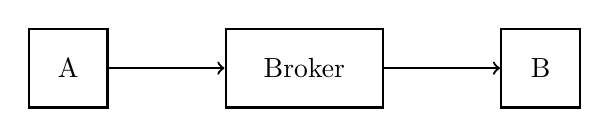
\begin{tikzpicture}[thick]
  \node(A) [draw,rectangle,minimum width=1cm,minimum height=1cm]{A};

  \begin{scope}[xshift=3cm]
    \node(Broker) [draw,rectangle,minimum width=2cm,minimum height=1cm]{Broker};
  \end{scope}

  \begin{scope}[xshift=6cm]
    \node(B) [draw,rectangle,minimum width=1cm,minimum height=1cm]{B};
  \end{scope}

  \draw[->] (A) edge (Broker)
            (Broker) edge (B);
\end{tikzpicture}

  \caption{Ten services exchanging messages via a broker}
  \label{fig:tikz:messageBroker}
\end{figure}

Message brokers offer a layer of abstraction to developers wishing to exchange
messages between services. Rather than contacting the service directly, messages
are relayed via the broker (Figure~\ref{fig:tikz:messageBroker}). This not only
reduced the number of connections required for application to exchange messages
(Figure~\ref{fig:tikz:complexBrokerMessaging}), but also simplifies service
discovery. Each service need only know the connection details for the message
broker, and the name of the queue/topic (Sections \ref{sub:queues} and
\ref{sub:topics}) to send/receive messages on. The locations of the services
sending/receiving messages through the broker no long matters - which removes
the need for complex service discovery protocols. Additionally, by decoupling
the sending and receiving of messages (Section~\ref{sub:pubsub}) brokers can act
as a buffer between communicating processes, preventing the receiving process
from becoming swamped by incoming messages (\gls{dos}).

\begin{figure}[ht]
  \centering
  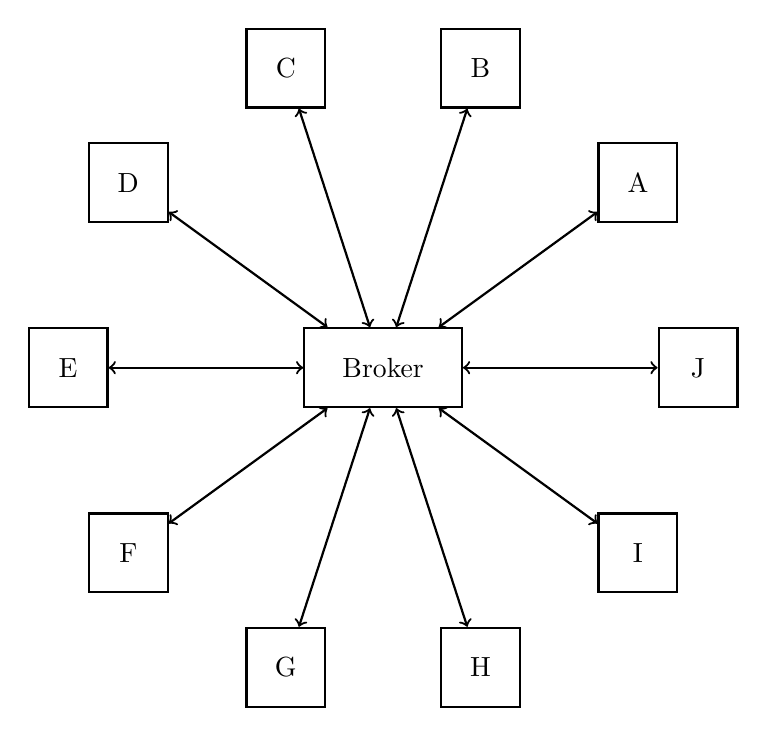
\begin{tikzpicture}[thick]

  % Draw nodes
  \foreach \t [count=\a] in {A,B,C,D,E,F,G,H,I,J}{
    \draw (\a*360/10: 4cm) node(\t)[draw,rectangle,minimum width=1cm,minimum height=1cm]{\t};
    }

  \begin{scope}
    \node(Broker) [draw,rectangle,minimum width=2cm,minimum height=1cm]{Broker};
  \end{scope}

  % Draw connections
  \foreach \t [count=\a] in {A,B,C,D,E,F,G,H,I,J}{
    \draw[<->] (\t) edge (Broker);
    }

\end{tikzpicture}

  \caption{Ten services exchanging messages via a broker}
  \label{fig:tikz:complexBrokerMessaging}
\end{figure}

\subsection{Pub/Sub}
\label{sub:pubsub}

Publish-subscribe is a software pattern, which describes the exchange of
messages between one-or-more producers (publishers), and one-or-more recipients
(subscribers). In a typical implementation, publishers send messages
(Section~\ref{sec:messages}) to a broker - with a named destination (either a
queue or topic). Subscribers register their interest ('subscribe') to these
named destinations, and receive all messages sent to said destinations, in a
manner dependent on whether the destination is a queue (see
Section~\ref{sub:queues}) or a topic (see Section~\ref{sub:topics}). This
pattern has several advantages, such as the ability for pub/sub infrastructure
to scale up to handle message routing for an entire datacenter, with relatively
little complexity. These advantages are explored in detail in
Section~\ref{sec:brokers}. The disadvantages of the pub/sub model are associated
with it's loose coupling - the model itself does not define a message format,
leaving the creation and updating of message contracts to the application
developer.\footnote{Although, as discussed in Section~\ref{sec:messages}, this
can also be an advantage}.

\subsection{Queues}
\label{sub:queues}

Queues are a standard feature of most programming languages, a core Computer
Science construct, and familiar to anyone who has ever been to a Post Office.
Queues are a \gls{fifo} data-structure, which delivers messages in the order
they were inserted into the queue. The other important features of queues in
terms of the pub/sub model, is that they can have multiple publishers, and
multiple subscribers. In the event of a queue having multiple subscribers,
messages are typically delivered in a 'round-robin' fashion - that is to say,
the next subscriber to receive a message will be the one who is ready to receive
a message that has received a message least recently.

A typical use of a Message
Queue may be the distribution of job information, where messages consist of
configuration for jobs, and worker applications subscribe to the queue this job
information is posted on. Once a worker has finished the job it's working on, it
received information for the next job off the queue. Each job is only ever
received by a single worker.\todo{Example code/diagram. Make this clearer}

\subsection{Topics}
\label{sub:topics}

Similar to Queues (Section~\ref{sub:queues}), topics are \gls{fifo} structures.
The key difference between topics and queues, is that whist queues deliver each
message to a single subscriber, topics deliver each message to \textbf{every}
subscriber. Each subscriber therefore receives a copy of each message sent to
the topic. A common use of topics, is the updating of information in a
distributed cache. Suppose a number of mobile phones maintained a cache of stock
prices, and rely on a pub/sub mechanism to receive the latest prices. Obviously,
a queue would be unsuitable for such a task, as it would only update the price
for a \textbf{single} subscriber. A topic would ensure that each stock price
published, would be sent to every mobile phone - updating the price for all
subscribers.\todo{Example code/diagram. Make this clearer}.

\subsection{Existing Brokers}
\label{sub:Existing Brokers}

Brief overview and comparison between some existing commercial/open-source
implementations, and their features.


\section{Broker Requirements}
\label{sec:requirements}

A message-broker is rather an unusual piece of software, due to the fact that is
has very few functional requirements.\todo{Elaborate?}

\subsection{Failure Handling}
\label{sub:Failure Handling}

The issue with gracefully handling communications failure in distributed systems
was illustrated in a 1988 paper by Xerox employees Andrew Birrell and Bruce
Nelson\cite{Birrell:1988:IRP:59309.59336}. They identified three different
semantics with which \glspl{rpc} could be executed:

\begin{description}
  \item[Exactly once] \hfill \\
    The ideal scenario is one in which messages are passed to their destination
    once, and exactly once. Typically, when failure does not occur during a
    message transfer this is trivial to assert - simply receiving an
    acknowledgement from the recipient of the message confirms this to be the
    case. Unfortunately, the same cannot be said when a response is not received
    from the recipient, for whatever reason (link failure/machine failure etc.).
    This is a typical illustration of the 'Two Generals
    Problem'\cite{Gray:1978:NDB:647433.723863} - and is extremely difficult to
    guard against. As a result - most messaging systems adopt one of the
    following behavioural models in the event of failure.
  \item[At most once] \hfill \\
    In the event that a message is lost without acknowledgement - no attempt is
    made to redeliver the message. This is used in situations where duplicated
    messages pose a risk to overall system integrity - for example in most
    financial systems.
  \item[At least once] \hfill \\
    In the event that a message is lost without acknowledgement, attempts to
    redeliver the message continue until successful receipt is acknowledged.
    This is typically used in situations where message delivery is deemed more
    important than message uniqueness/ordering. For example, if the
    unacknowledged message is intended to trigger a cache refresh in the
    recipient system - the fact that the refresh may occur multiple times may be
    insignificant next to the risk that the refresh does not happen at all.
\end{description}

\subsection{Network Bandwidth Utilisation}
\label{sub:Network Bandwidth Utilization}

In many situations (and in \gls{iot} devices in particular) network bandwidth is
a limiting resource. Message compression can be used in certain situations to
reduce overall bandwidth utilisation of the broker - at the cost of increased
computational load on both the broker and consumer.

\subsection{Network latency}
\label{sub:Network latency}

Devices experiencing high degrees of network latency can have tremendous impact
on the overall \gls{rtt} of a given message. This can be compensated for through
intelligent packet stuffing (such as Nagel's algorithm)/jumbo frames (if
supported) by the network - all of which reduce the amount of overhead
experienced by each message.

\subsection{Network packet loss}
\label{sub:Network packet loss}

On networks experiencing a high rate of packet loss - error correcting protocols
like TCP can help ensure packet delivery at the IP layer. Additionally,
check-summing the messages can help guard against message corruption through
lost packets.

\subsection{Message power cost}
\label{sub:Message power cost}

Especially relevant for \gls{iot} and low-power devices - the amount of power
consumed whilst exchanging messages (which is directly linked to the number of
CPU cycles required to transmit/receive each message) can be an important
consideration when designing an applications. Message attributes which can
affect this include:

\begin{itemize}
  \item Message compression
  \item Message size
  \item IP Protocol
  \item Network conditions (requiring re-transmits/computing checksums etc.)
\end{itemize}

\subsection{Message throughput}
\label{sub:Message throughput}

Finally - the most obvious performance metric of a broker - the number of
messages it can process per second. This is impacted by all of the above
requirements, and can be maximised through the use of small, cheap messages,
with as little overhead as possible. Network protocol can make a large
difference here - with something like UDP being extremely cheap to send over the
wire (if inherently unreliable).

\section{GoLang}
\label{sec:GoLang}

\todo[inline]{Overview of GoLang}

\subsection{What is GoLang?}
\label{sub:What is GoLang?}

As mentioned in the introduction (Section~\ref{sec:background}), GoLang is a
compiled, statically-typed language developed in part out of the authors
frustrations with using more traditional languages, such as Java and C++, to
develop network applications\cite{kenThompsonInterview}. Announced to the
general public in 2009, GoLang was internally developed at Google to resolve the
common criticisms with other popular languages at the time of development - a
prime example being the long compilation times involved with working in
languages such as C++\footnote{\url{http://stackoverflow.com/a/318440/1657432}}.
One of the founding principals of Go was simplicity, and ease of
maintainability\cite{lessIsExponentiallyMore} - even at the expense of
performance in some areas. As such, Go has a relatively light core feature-set
compared with most other 'network-oriented languages', and contains creature
comforts not found in other performance-oriented languages like C++, such as
Garbage Collection - something which has typically been the sole preserve of
languages with an interpreted runtime, such as Java, Ruby and Python. However,
due to its nature as a compiled language, Go still outperforms these
'traditional languages' in a number of standard
benchmarks\footnote{\url{https://benchmarksgame.alioth.debian.org/u64q/go.html}}
which, combined with the multitude of built-in concurrency features
(Section~\ref{sub:golangConcurrency}) make Go an extremely compelling language
for developing networked infrastructure code, such as a message broker.

\subsection{Concurrency vs Parallelism}
\label{sub:concurrencyparallelism}

\todo[inline]{Why do we need either?}

Confusion often exists as to the relationship between parallelism and
concurrency, thanks in part to their often similar dictionary definitions:

\begin{description}
  \item[Concurrent] \hfill \\
  Going on side by side, as proceedings; occurring together, as events or
  circumstances; (\textit{source: OED})
  \item[Parallelism] \hfill \\
  Concurrent or contemporary; existing in the same period of time.
  (\textit{source: OED})
\end{description}

However, as they relate to Computer Science, parallelism and concurrency are not
at all the same. A concurrent task is one that has been designed to be
independent of other tasks and which is interrupt-able. Concurrent tasks
\emph{may or may not} be run in parallel with other concurrent tasks, and have
the potential to decrease the real-world-time taken to perform a set of actions,
even if executed on single-threaded (non-parallel) hardware. \\

An real-world analogy - suppose the organisers of a draughts tournament wish to
give 10 amateur players the opportunity to play a game with a professional
player, and wish to conduct these games in as time-efficient a manner as
possible. There are multiple ways the tournament could be run. \\

The professional player could sit down with each of the ten amateurs, and play
him/her to completion - before moving on to the next amateur. This is synonymous
with \textbf{sequential} code execution. Assuming each game takes 10 minutes to
complete, and that the time taken to transition from one game to another is 6
seconds. $$6 \text{seconds} * 10 \approx 1 \text{minute}$$
The time taken to complete the tournament is therefore 101 minutes (1 hour, 41
minutes). This is the worst case scenario. \\

An alternative method of running the tournament would be to get the professional
to play all 10 games \textbf{concurrently}. In this scenario, she would play
a move against one opponent, before immediately moving on to the next game -
leaving the amateur player to make his move. Assume that the professional player
takes 6 seconds to play each move and, as before, takes 6 seconds to transition
between games. With 10 amateur players, it will take approximately 120 seconds
before she returns to her starting seat. Now assume that each amateur player
takes 45 seconds to take his/her turn. Based on the 10 minute timer from the
serial game - each game will last for 11 rounds.
$$(10 * 60) / (45 + 6) \approx 11$$
The total time for the game is therefore
$$(11 * \text{time\_taken\_per\_move} + 11 * \text{transition\_time}) = (11 * 51) + (11 * 60) = 1221 \text{seconds}$$
This equates to 20 minutes, and 21 seconds - a dramatic improvement over the
sequential method. \\

Now we can look at the effect of simple \textbf{parallelism} on the tournament
time. Assuming we return to the sequential tournament method, but invite a
second professional player to the match. The effects of this are rather
obviously - playing two games at once will half the time taken to complete all
games, which will now take 55 minutes to carry out. $$101/2 \approx 55$$
However, note that we not only require twice as many 'resources' (in this case,
professional draughts players) as before, but took \emph{longer} to complete the
tournament than the concurrent method. \\

\todo{Mention (Javascript) callbacks} \\

\todo[inline]{Async IO vs multiple threads}

\subsection{Concurrency in GoLang}
\label{sub:golangConcurrency}

\subsection{Why do we need concurrency?}
\label{sub:whyConcurrency}

A message broker operates in, what is an inherently parallel environment. As
shown in Figure~\ref{fig:tikz:complexBrokerMessaging}, a broker is expected to
hold a great many 'conversations' with clients at any one moment in time. These
clients will be sending new messages, expecting to receive published messages,
creating/deleting queues and topics - all at the same time. As mentioned in
Section~\ref{sec:requirements}, these client requests need to be serviced in a
timely manner. Whilst a sequential approach to designing a broker may well work
in simple environments, this approach simply does not scale to the levels of
enterprise message brokers, which deal with thousands of message per second,
serving hundreds of clients.

One approach to dealing with this environmental parallelism, is to use
multi-threading. In a traditional language like Java, creating a separate thread
for dealing with each client would improve the response times for individual
clients, as well as allow the broker to take advantage of modern, multithreaded
hardware. There exist, however, two big issues with this approach. In more
traditional multi-threaded languages.

\paragraph{Memory footprint} \mbox{}\\

\begin{figure}[H]
  \centering
  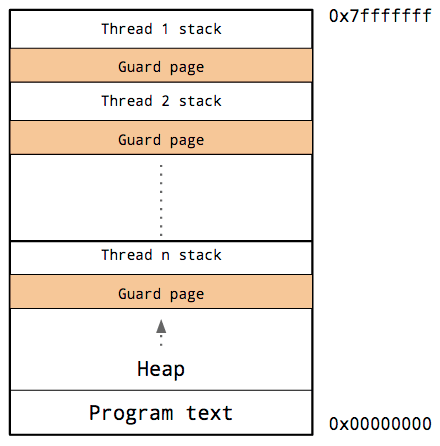
\includegraphics[width=0.5\textwidth]{figures/threads}
  \caption{Traditional thread memory model \cite{performanceWithoutTheEventLoop}}
  \label{fig:threadMemoryModel}
\end{figure}

Threads have a fairly large memory footprint. Java threads, for example, are
allocated with roughly \SI{512}{\kibi\byte} of stack memory. Each thread stack
is bounded by a \emph{guard page} - to prevent the stack from overwriting the
heap, as shown in Figure~\ref{fig:threadMemoryModel}, and which is typically
\SI{4}{\kibi\byte} in size. \SI{512}{\kibi\byte} is a fairly large stack
allocation, due to the fact that it is impossible to know at 'spawn time' how
much stack memory a thread is going to use, and it is not possible to resize the
stack at a later time. Assuming we were to use a single thread for each client,
a broker with 1000 clients would consume roughly \SI{512}{\mebi\byte} of memory
\emph{just} for the client threads.

\begin{figure}[H]
  \centering
  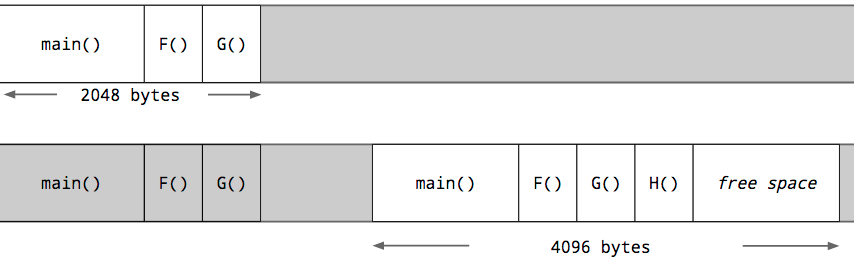
\includegraphics[width=0.8\textwidth]{figures/stack-growth}
  \caption{Goroutine memory model \cite{performanceWithoutTheEventLoop}}
  \label{fig:goMemoryModel}
\end{figure}

By comparison, Goroutines start life with a small stack, allocated from the heap
memory (Figure~\ref{fig:goMemoryModel}). Rather than using a guard page to
detect stack overflow, each time the function is called, a small piece of code
tests that there is sufficient stack space for the function to run. In the event
that there is insufficient space a new, bigger stack is allocated from the heap,
copy the contents of the old stack over, and free the original stack memory.
This resizing is possible because Go allocates stack space within the heap
itself, rather than a separate chunk of memory. Because resizing is possible, Go
can afford to allocate a much smaller initial stack for Goroutines, as the
penalty for stack overflow is a (relatively mild) performance hit, rather than
an application crash under the previous model
(Figure~\ref{fig:threadMemoryModel}). As of Go 1.4, the default starting size of
a Goroutines stack is
\SI{2}{\kibi\byte}\footnote{\url{https://golang.org/doc/go1.4\#runtime}}. Using
the same example from above, a 1000-client broker using Goroutines would require
\SI{2}{\mebi\byte} of memory, or a $\sim250\%$ saving over the traditional
thread model.

\paragraph{Context switching} \mbox{}\\

\todo[inline]{Message broker functions - blocking vs non-blocking IO}

\todo[inline]{GoRoutines/Channels etc.}
